\pagestyle{romanstyle}
\pagenumbering{Roman}
%%%%% ABSTRACT
\begin{abstract}
	This study investigates the entanglement properties of a 1D lattice modeled by the Heisenberg XY model with the inclusion of Dzyaloshinskii-Moriya interaction (DMI). We analyze the concurrence between qubits under various configurations of the DMI constant \(D\), the anisotropy parameter \(\delta\), and the correction factor \(\gamma\). Both 2-qubit and 3-qubit systems are considered to understand the influence of these parameters on quantum entanglement. Our findings reveal that the DMI generally enhances the entanglement between qubits, as indicated by increased concurrence values. However, the anisotropy parameter \(\delta\) introduces a competing effect that can reduce entanglement, particularly when \(\delta\) is increased. The results provide insight into how these parameters can be tuned to control entanglement in quantum systems, which is crucial for applications in quantum information processing and the design of quantum materials.


\end{abstract}

\underline{\textbf{Keywords :}} Entanglement, Dzyaloshinskii-Moriya interaction, Heisenberg XY model

\newpage
%%%% Acknowledgements
\section*{Acknowledgements}
I would like to begin by expressing my deep gratitude to Guillermo Romero, my tutor, Associate Professor in the Physics Department at the Universidad de Santiago de Chile, and researcher at the Center for the Development of Nanoscience and Nanotechnology (CEDENNA), for giving me such a warm welcome to Chile. I am extremely thankful for his support and for providing me with the opportunity to enjoy this unforgettable experience, which combined fascinating research with the discovery of Chile.

I would also like to extend my thanks to my academic tutor, Pascal Lafon, for his supervision and support.

Finally, I wish to acknowledge my family and all the people I met in Chile.
\begin{center}
	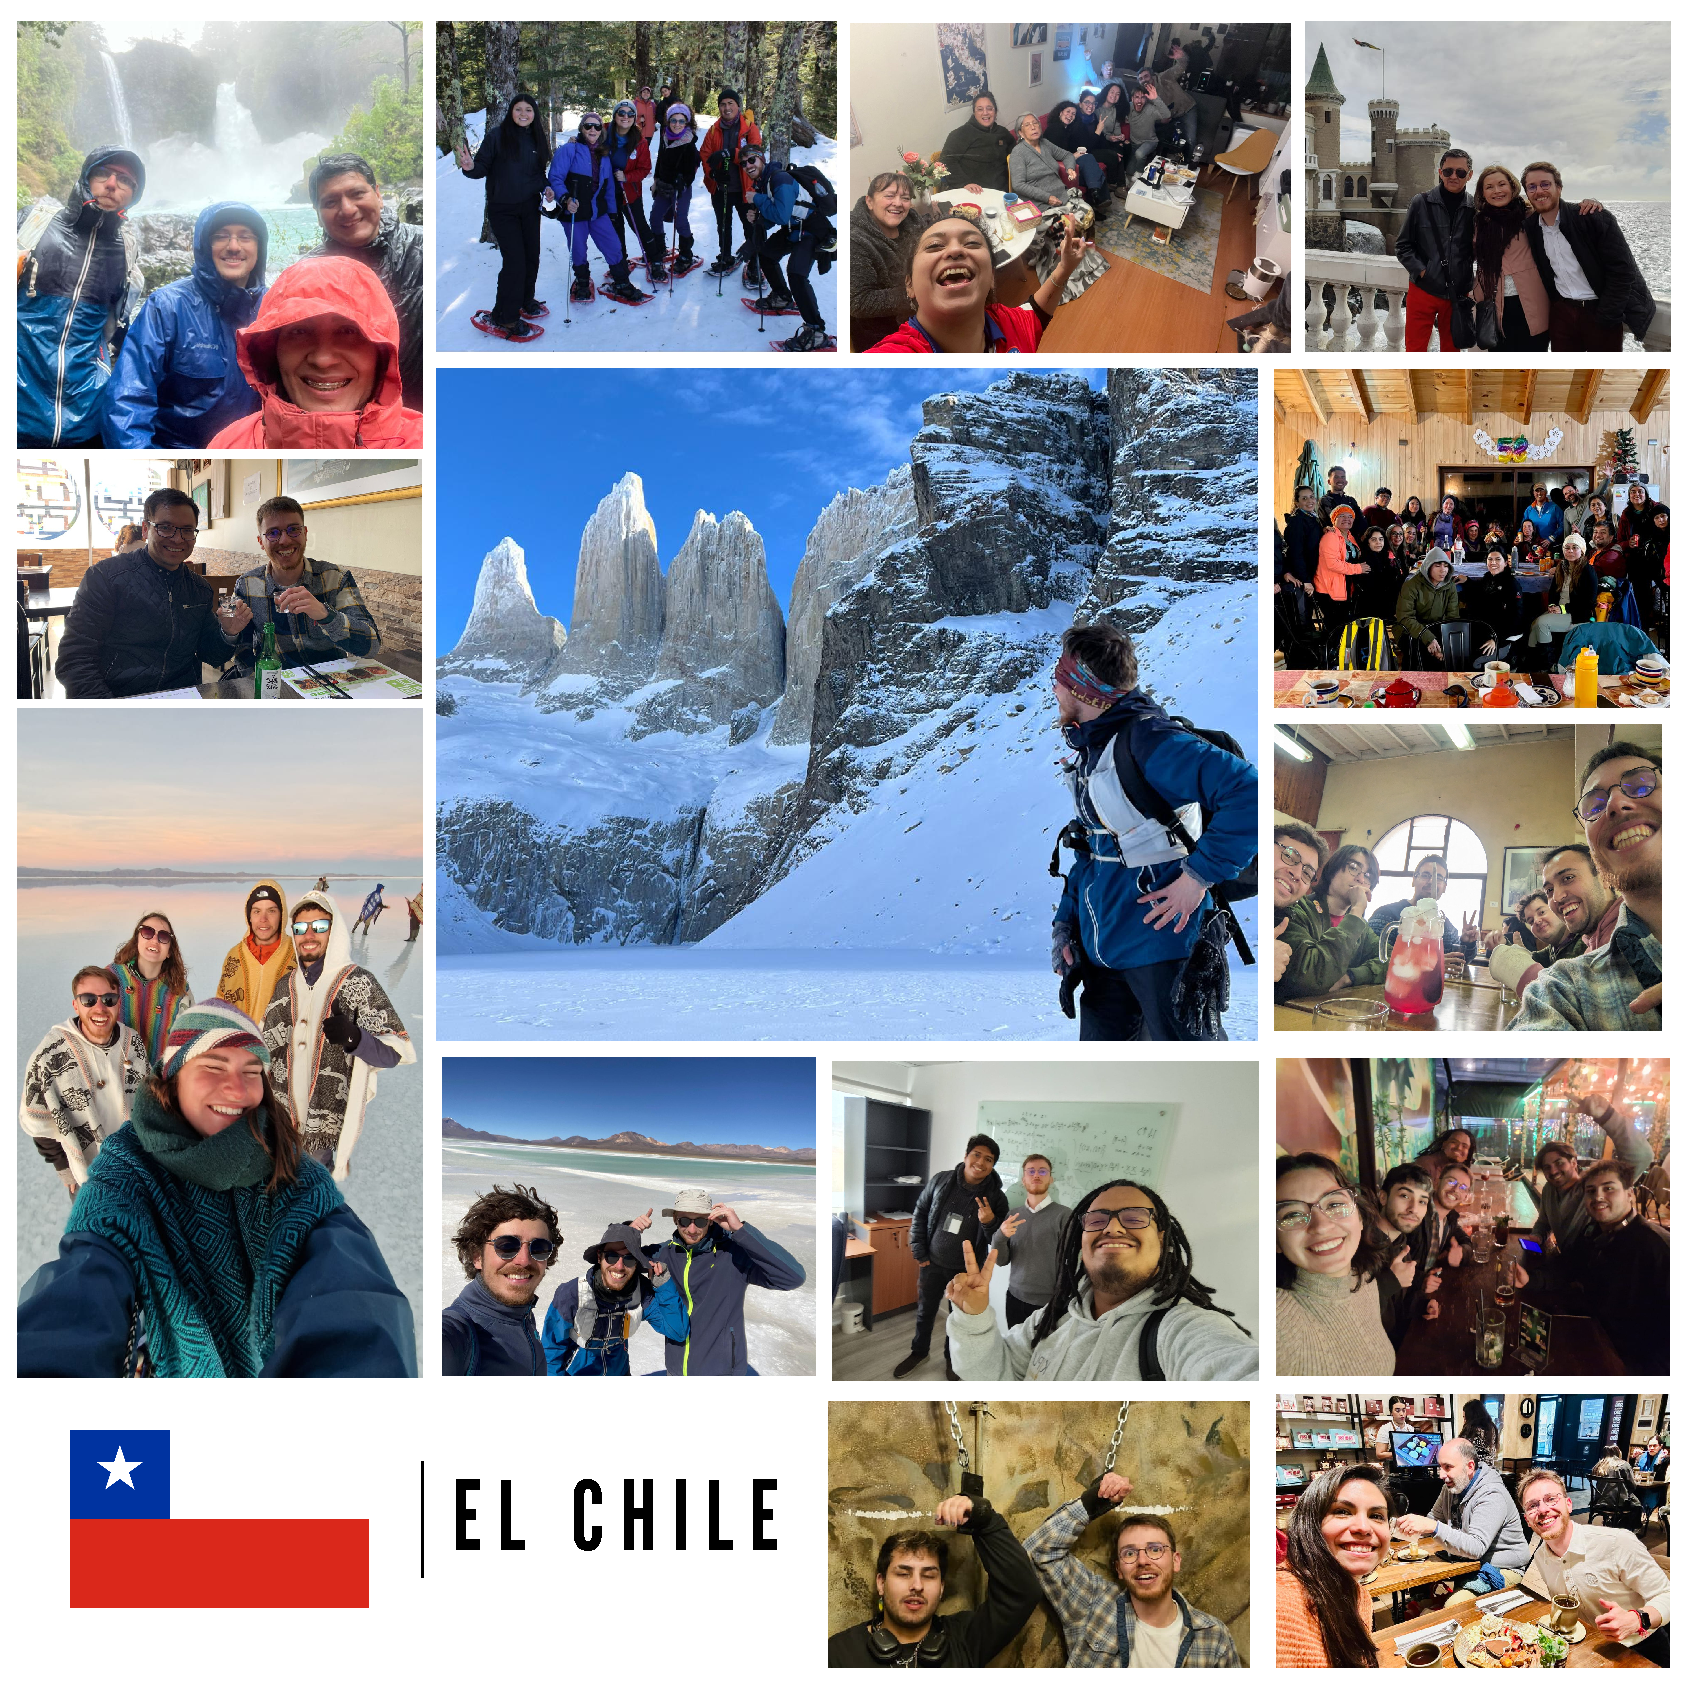
\includegraphics[width=0.8\linewidth]{formal_part/BILAN Chile.pdf}
\end{center}

\newpage



\newpage
%%%% List of tableofcontents

		
\startcontents[sections]
\printcontents[sections]{l}{1}{\setcounter{tocdepth}{2}}

\newpage

		\listoffigures




